\subsection{Matrix Multiplication}\label{ssec:matrix_mult}

\begin{figure*}[t]
    \centering
    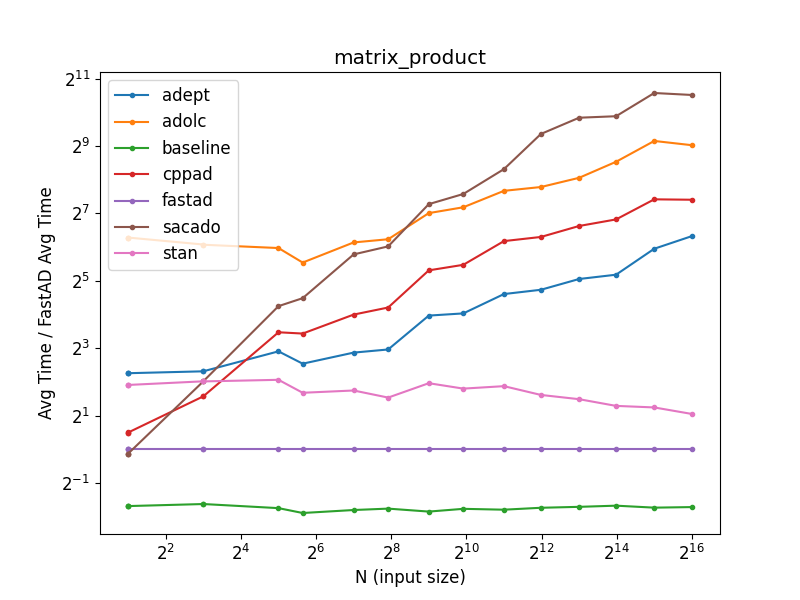
\includegraphics[width=0.8\textwidth]{figs/matrix_product_fig.png}
    \caption{%
        Matrix multiplication benchmark of other libraries against FastAD 
        plotted relative to FastAD average time.
    }\label{fig:matrix_mult}
\end{figure*}

For this benchmark, all matrices are square matrices of the same size.
In order to have a scalar target function,
we add another step of adding all of the entries of the matrix multiplication, i.e.
\[
    f(A, B) = \sum\limits_{i=1}^{K} \sum\limits_{j=1}^{K} {(A \cdot B)}_{ij}
\]
Fig.~\ref{fig:matrix_mult} shows the benchmark results.

FastAD is still the fastest library for all values of $N$, 
but Stan performs much closer to FastAD than in the previous examples.
All other libraries consistently take longer than both FastAD and Stan as $N$ increases.
Towards the end at around $N=2^{14}$, 
Stan is about $ 2$ times slower.
For moderate sized $N \in [2^{8}, 2^{10}]$, Stan is about $ 3$ times slower.

This example really highlights the benefits of vectorization.
As noted in Section~\ref{ssec:vectorization},
this was the one benchmark example where Stan was able to produce vectorized code,
which is consistent with Figure~\ref{fig:matrix_mult} 
that Stan is the only library that has the same 
order of magnitude as FastAD.
Other libraries did not produce vectorized code.

The comparison with the baseline shows that FastAD takes $ 3.27$ times longer.
Note that forward-evaluation requires one matrix multiplication between two $K\times K$ matrices,
and backward-evaluation additionally requires two matrix multiplications of the same order,
one for each adjoint:
\begin{align*}
    \frac{\partial f}{\partial A} 
    &= \frac{\partial f}{\partial (A\cdot B)} \cdot B^T, \,
    \frac{\partial f}{\partial B} 
    = A^T \cdot \frac{\partial f}{\partial (A\cdot B)}
\end{align*}
Hence, in total, one AD evaluation requires three matrix multiplications between two $K\times K$ matrices.
If we approximate a manually-written gradient computation to take 
three times as long as the baseline (one multiplication), 
FastAD time relative to this approximated time
is $\frac{3.27}{3} = 1.09$.
This shows then that FastAD only has about $ 9\%$ overhead 
from a manually-written code, which is extremely optimal.
